% ============================================================================
% Articulo (compatible con Overleaf) que resuelve los 4 retos practicos de
% vision clasica de la Guia 1 del curso Vision por Computador Avanzada
% (Doctorado en Innovacion e Ingenieria). Cada reto cierra con un breve
% comentario -- no el eje del documento -- sobre su relacion con la linea
% de investigacion doctoral del autor (marco DOE para evaluar SLAM).
%
% Compilacion local (VSCode + LaTeX Workshop, o linea de comandos):
%   pdflatex main.tex
%   bibtex main
%   pdflatex main.tex
%   pdflatex main.tex
%
% En Overleaf: subir esta carpeta paper/ completa (main.tex, referencias.bib,
% figuras/) y compilar con pdfLaTeX + BibTeX (configuracion por defecto).
%
% Si el articulo se preparara para una revista/conferencia especifica
% (p. ej. IEEE RA-L, IROS, ICRA), reemplazar \documentclass{article} por la
% plantilla oficial correspondiente (p. ej. IEEEtran), conservando el
% contenido de cada seccion.
% ============================================================================
\documentclass[11pt]{article}

\usepackage[utf8]{inputenc}
\usepackage[spanish]{babel}
\usepackage{graphicx}
\usepackage{amsmath}
\usepackage{mathtools}
\usepackage{booktabs}
\usepackage{hyperref}
\usepackage{natbib}
\usepackage[margin=2.5cm]{geometry}
\usepackage{algorithm}
\usepackage{algpseudocode}

\title{Ejercicios Fundamentales de Visión por Computador Clásica:\\
Representación Matricial, Convoluciones, Segmentación por Color\\
y Filtrado de Ruido\\
\large Entregable práctico -- Guía 1, curso Visión por Computador Avanzada}

\author{Milton Alvarado \\ \small mealvarado@elpoli.edu.co \\
\small Doctorado en Innovación e Ingeniería, Politécnico Colombiano Jaime Isaza Cadavid}
\date{\today}

\begin{document}
\maketitle

\begin{abstract}
Este documento presenta la solución a los cuatro retos prácticos de visión
por computador clásica planteados en la Guía 1 del curso \emph{Visión por
Computador Avanzada} (Doctorado en Innovación e Ingeniería): (1)
representación matricial de una imagen sintética y caracterización
estadística manual frente a vectorizada con Numpy; (2) convoluciones con
kernels de bordes (Sobel) y de suavizado (gaussiano) implementadas celda a
celda en una hoja de cálculo; (3) extracción y caracterización estadística
por color de regiones de interés en una imagen a color; y (4) eliminación
de ruido impulsivo (\emph{salt~\&~pepper}) mediante filtrado por
convolución, comparando cuatro implementaciones manuales (media, moda,
mediana, gaussiana) con sus equivalentes de OpenCV. Cada reto se resolvió
con código e implementaciones propias del autor, verificado de forma
independiente, y se acompaña de un análisis cuantitativo de los resultados
y de las conclusiones solicitadas por la guía. Como valor agregado, el
cuarto reto incorpora una comparación estadística formal entre los filtros evaluados, un análisis ANOVA  de un
factor para respaldar estadisticamente la diferencia del efecto sobre la imagen y la prueba post-hoc de Tukey para encontrar el que tiene mejor desempeño usando la métrico SSIM como variable de salida como un primer
ensayo de la línea de trabajo doctoral del autor orientada a evaluar
algoritmos SLAM mediante Diseño de Experimentos (DOE).
\end{abstract}

\section{Introducción}
Este documento corresponde a la entrega del componente evaluable de visión
clásica del curso \emph{Visión por Computador Avanzada} (Doctorado en
Innovación e Ingeniería, Politécnico Colombiano Jaime Isaza Cadavid), de
acuerdo con los cuatro retos definidos en la Guía~1 de la asignatura: (1)
\emph{Matrices a imágenes}, (2) \emph{Convoluciones en Excel}, (3)
\emph{Colores}, y (4) \emph{Convoluciones para filtrado}. Cada reto se
resuelve siguiendo los pasos solicitados en la guía (Secciones
\ref{sec:reto1}--\ref{sec:reto4}), con implementaciones propias del autor,
resultados verificados de forma independiente, y evidencia reproducible
disponible en un repositorio público (Sección~\ref{sec:datos-codigo}).

Adicionalmente a lo solicitado en la guía, cada reto cierra con un breve
comentario sobre su relación con la línea de investigación doctoral del
autor -- un marco metodológico basado en Diseño de Experimentos (DOE)
\citep{montgomery2019design} para evaluar el desempeño de algoritmos SLAM
\citep{cadena2016past} --, dado que varios de los conceptos aquí ejercitados
(medición reproducible de tiempos, caracterización estadística de variables
de respuesta, comparación formal de "tratamientos" mediante ANOVA) son
piezas de infraestructura reutilizables en dicho marco. Estos comentarios
son deliberadamente breves: el cuerpo de este documento se centra en
resolver y documentar cada reto conforme a los criterios de evaluación de
la guía, no en el marco doctoral, que queda solo esbozado como proyección
en las Conclusiones (Sección~\ref{sec:conclusiones}).

\section{Marco teórico}
Los cuatro retos se apoyan en conceptos estándar de procesamiento digital
de imágenes \citep{gonzalez2018digital}: la representación de una imagen
como matriz de intensidades y su caracterización mediante estadísticos
descriptivos (Reto 1); el operador de convolución y los kernels de Sobel y
de suavizado gaussiano (Reto 2); la representación de color en el espacio
BGR y su caracterización estadística por región (Reto 3); y el filtrado no
lineal (mediana, moda) frente al lineal (media, gaussiana) para eliminar
ruido impulsivo, evaluado aquí mediante el índice de similitud estructural
(SSIM) \citep{wang2004ssim} (Reto 4). Estos mismos bloques de
construcción -- kernels de convolución, descriptores estadísticos de
región, filtrado de ruido -- son además los que emplean internamente los
algoritmos de SLAM visual (p.~ej.\ ORB-SLAM2 \citep{murartal2017orbslam2})
y de odometría visual \citep{scaramuzza2011visualodometry}, lo que motiva
tratarlos aquí con detalle de primer principio en vez de como funciones de
caja negra de una librería.

\section{Datos y disponibilidad de código}
\label{sec:datos-codigo}
Para los cuatro retos se trabajó de forma local (VSCode) con respaldo en
control de versiones Git/GitHub, en lugar de Google Colab/Drive -- sustitución
explícitamente autorizada por el profesor del curso, y que cumple el mismo
propósito de la guía (evidencia versionada y recuperable del proceso
completo). El código completo, con instrucciones de ejecución y pruebas
automatizadas, está disponible públicamente en un repositorio de GitHub
\citep{alvarado2026repo}\footnote{URL del repositorio pendiente de
publicación final: \url{<URL\_DEL\_REPOSITORIO>}. Actualizar esta nota y la
entrada \texttt{alvarado2026repo} en \texttt{referencias.bib} en cuanto el
repositorio quede publicado (ver \texttt{paper/borrador\_articulo.md} para
el procedimiento sugerido, incluyendo el registro opcional de un DOI
permanente vía Zenodo).}.

Los datos usados en los Retos 1, 3 y 4 (Secciones
\ref{sec:reto1}, \ref{sec:reto3} y \ref{sec:reto4}) son sintéticos:
la matriz aleatoria del Reto 1 se genera con semilla fija
($s=42$) para garantizar reproducibilidad exacta, y la imagen a color usada
en los Retos 3 y 4 es una escena sintética generada mediante IA
generativa de imágenes (Google Gemini), diseñada para emular, con fines
ilustrativos y de prueba de concepto, un banco de pruebas de calibración de
cámara/color típico de un laboratorio de robótica -- no corresponde a una
fotografía capturada de un entorno físico real. Los resultados cuantitativos
de esos retos (estadísticas por canal, análisis de filtrado) se
calcularon sobre los valores de píxel reales de esa imagen, y las
conclusiones sobre el comportamiento de los algoritmos evaluados son válidas
independientemente del origen sintético de la imagen; la validación de
dichas conclusiones sobre escenas físicas reales queda como trabajo futuro
(Sección~\ref{sec:conclusiones}).

\section{Desarrollo de los retos}

\subsection{Reto 1: Matrices a imágenes}
\label{sec:reto1}

\subsubsection{Método}
Siguiendo el procedimiento de la guía, se generó -- sin librerías de
cómputo matricial, usando únicamente la librería \texttt{random} de Python
y listas de listas -- una matriz de $1000\times 1000$ valores enteros
aleatorios en el rango $[0,255]$ (equivalente a \texttt{uint8}). Sobre esa
matriz se implementó, también sin librerías especializadas, una función
que recorre la matriz ya aplanada a un vector unidimensional y calcula
mínimo, máximo, media y desviación estándar mediante las fórmulas
explícitas $\bar{x} = \frac{1}{n}\sum_i x_i$ y
$\sigma = \sqrt{\frac{1}{n}\sum_i (x_i - \bar{x})^2}$, con semilla fija
$s=42$ para garantizar reproducibilidad exacta entre corridas. Se midió con
\texttt{time.time()} el tiempo total del proceso, desde la creación de la
matriz hasta la obtención de estos cuatro estadísticos.

El vector aplanado se guardó en un archivo de texto plano (\texttt{.csv})
en disco. El curso autoriza explícitamente trabajar de forma local con
respaldo en Git/GitHub como sustituto de subir el archivo a Google Drive y
volver a leerlo desde Colab (paso solicitado por la guía); esa sustitución
y el archivo generado quedan documentados en el repositorio versionado
(Sección~\ref{sec:datos-codigo}). Tras leer el archivo con
\texttt{numpy.loadtxt} y reconstruir la matriz original, se recalcularon
los mismos cuatro estadísticos con Numpy y se volvió a medir el tiempo del
proceso completo, para comparar contra la versión manual. Finalmente, la
matriz se visualizó como imagen en escala de grises con Matplotlib. Código
completo en
\texttt{retos/reto1\_matrices\_a\_imagenes/version\_final/reto\_1.py} del
repositorio.

\subsubsection{Resultados}

La Tabla~\ref{tab:reto1-stats} resume la comparación entre ambas
implementaciones sobre la misma matriz (los valores estadísticos
coinciden exactamente, salvo precisión numérica de punto flotante).

\begin{table}[h]
\centering
\caption{Comparación de estadísticos y tiempos entre la implementación manual (Python puro) y Numpy, sobre una matriz de $1000\times1000$ valores (semilla $s=42$).}
\label{tab:reto1-stats}
\begin{tabular}{lrr}
\toprule
Métrica & Manual (Python puro) & Numpy \\
\midrule
Mínimo & 0 & 0 \\
Máximo & 255 & 255 \\
Media & 127.45 & 127.45 \\
Desviación estándar & 73.92 & 73.92 \\
\midrule
Tiempo total del proceso (s) & 0.4848 & 0.0752 \\
\bottomrule
\end{tabular}
\end{table}

El proceso manual resultó aproximadamente $6.4\times$ más lento que el
proceso con Numpy. El factor exacto de aceleración varía con el hardware
(se observaron valores entre $4.3\times$ y $6.7\times$ en distintas
corridas y máquinas), pero la conclusión cualitativa --Numpy sensiblemente
más rápido-- se sostuvo en todos los casos. La Figura~\ref{fig:reto1-imagen}
muestra la matriz resultante visualizada como imagen en escala de grises.

\begin{figure}[h]
\centering
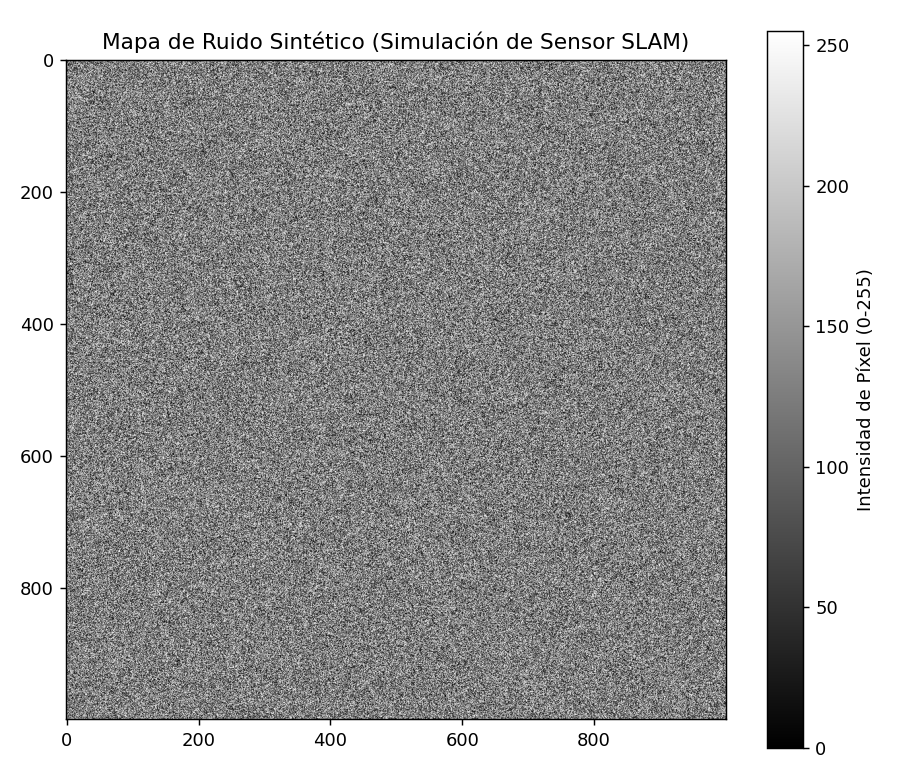
\includegraphics[width=0.55\textwidth]{figuras/reto1_mapa_ruido_final.png}
\caption{Matriz de $1000\times1000$ (semilla $s=42$) visualizada como mapa de ruido sintético en escala de grises.}
\label{fig:reto1-imagen}
\end{figure}

Como extensión propia más allá de lo pedido por la guía, se diseñó un
experimento de un factor (tamaño de la matriz $N$, con
$N \in \{100,300,500,800,1000\}$ y 5 repeticiones por nivel) para
caracterizar el efecto de $N$ sobre el tiempo de ejecución del proceso
manual. La Figura~\ref{fig:reto1-experimento}
muestra la curva de respuesta resultante (media $\pm$ desviación estándar
del tiempo, por nivel), consistente con el crecimiento cuadrático $O(N^2)$
esperado.

\begin{figure}[h]
\centering
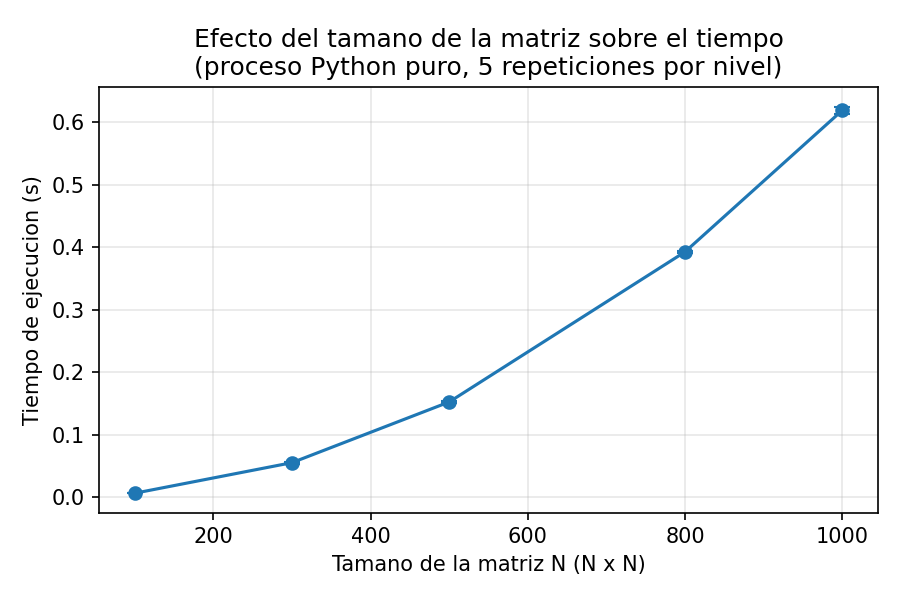
\includegraphics[width=0.6\textwidth]{figuras/reto1_experimento_tamano.png}
\caption{Efecto del tamaño de la matriz $N$ sobre el tiempo de ejecución del proceso manual (5 repeticiones por nivel).}
\label{fig:reto1-experimento}
\end{figure}

\subsubsection{Análisis y conclusiones}
Los estadísticos calculados manualmente y con Numpy coinciden exactamente
(salvo precisión de punto flotante), lo que confirma que la implementación
manual es correcta. La diferencia de tiempos ($\sim 6.4\times$ más lento en
Python puro) es la esperada: Numpy vectoriza las operaciones aritméticas,
evitando el recorrido explícito elemento a elemento que exige la
implementación manual; el experimento adicional de la
Figura~\ref{fig:reto1-experimento} confirma además el crecimiento
cuadrático $O(N^2)$ del proceso manual al variar el tamaño $N$ de la
matriz, mientras que Numpy escala de forma mucho más suave. Esta
comparación -- una variable de respuesta cuantitativa (tiempo), medida bajo
condiciones controladas y reproducibles (semilla fija) -- es, de forma
incidental, el mismo tipo de comparación de "tratamientos" (aquí,
implementaciones) que la línea de investigación doctoral del autor busca
formalizar más adelante para comparar algoritmos SLAM (Sección~\ref{sec:conclusiones}).

\subsection{Reto 2: Convoluciones en Excel}
\label{sec:reto2}

\subsubsection{Método}
Se construyó, en una hoja de cálculo, una matriz base de $30\times 30$
celdas que simula una escena mínima con una esquina a detectar: una región
de fondo con valores aleatorios entre 0 y 10 (\texttt{ALEATORIO.ENTRE(0;10)}),
un borde de una celda de ancho que actúa como zona de penumbra (transición
de intensidad intermedia), y una esquina de mayor intensidad (hasta 255)
que constituye el objeto a detectar. Se usó deliberadamente una función
aleatoria para el fondo y la penumbra --en vez de dejar un valor teórico
constante-- para introducir una variabilidad tipo ruido de sensor, más
representativa de una imagen real que una escena perfectamente uniforme.
Siguiendo la guía, las celdas se colorearon con formato condicional de
escala de grises (0 = negro, 127 = gris medio, 255 = blanco), y se
definieron y probaron varios kernels $3\times 3$: dos kernels de borde
(Sobel horizontal $K_x$ y vertical $K_y$) y un kernel de suavizado
(gaussiano), los tres tomados de la literatura estándar de procesamiento
de imágenes \citep{gonzalez2018digital}. Los dos Sobel se combinaron como
$|G_x|+|G_y|$ para obtener el mapa de bordes. El mismo procedimiento
(Sobel-H, Sobel-V, combinado) se repitió sobre una versión de la matriz
suavizada previamente con el kernel gaussiano $3\times 3$ ($\sigma\approx
0{,}8$), para comparar la sensibilidad del operador de Sobel al ruido de
fondo con y sin un preprocesamiento de suavizado. El Algoritmo~\ref{alg:conv3x3}
describe, de forma general, la operación de filtrado por vecindad
deslizante que subyace tanto a este reto como al Reto 4
(Sección~\ref{sec:reto4}): la única diferencia entre ambos es la función de
agregación $f$ aplicada a cada vecindad.

\begin{algorithm}
\caption{Filtrado por vecindad deslizante $3\times 3$}
\label{alg:conv3x3}
\begin{algorithmic}[1]
\Require Imagen $I$ de tamaño $H \times W$; función de agregación $f$
\Statex \hspace{1.5em} ($f$ = suma ponderada por kernel $K$, en este reto;
\Statex \hspace{1.5em} $f \in \{\text{media}, \text{mediana}, \text{moda}\}$ en el Reto 4)
\Ensure Imagen filtrada $I'$
\For{$i \gets 1$ \textbf{hasta} $H-2$}
    \For{$j \gets 1$ \textbf{hasta} $W-2$}
        \State $V \gets I[i-1{:}i+2,\, j-1{:}j+2]$ \Comment{vecindad $3\times 3$ centrada en $(i,j)$}
        \State $I'[i,j] \gets f(V)$
    \EndFor
\EndFor
\State \Return $I'$
\end{algorithmic}
\end{algorithm}

Para el kernel gaussiano, $f(V) = \left(\sum V \odot K\right) / \sum K$, con
$K = \begin{bsmallmatrix}1&2&1\\2&4&2\\1&2&1\end{bsmallmatrix}$; para Sobel,
$f(V) = \sum V \odot K_x$ (análogamente para $K_y$), y la magnitud de borde
reportada es $|G_x| + |G_y|$.

\subsubsection{Resultados}

\begin{figure}[ht]
\centering
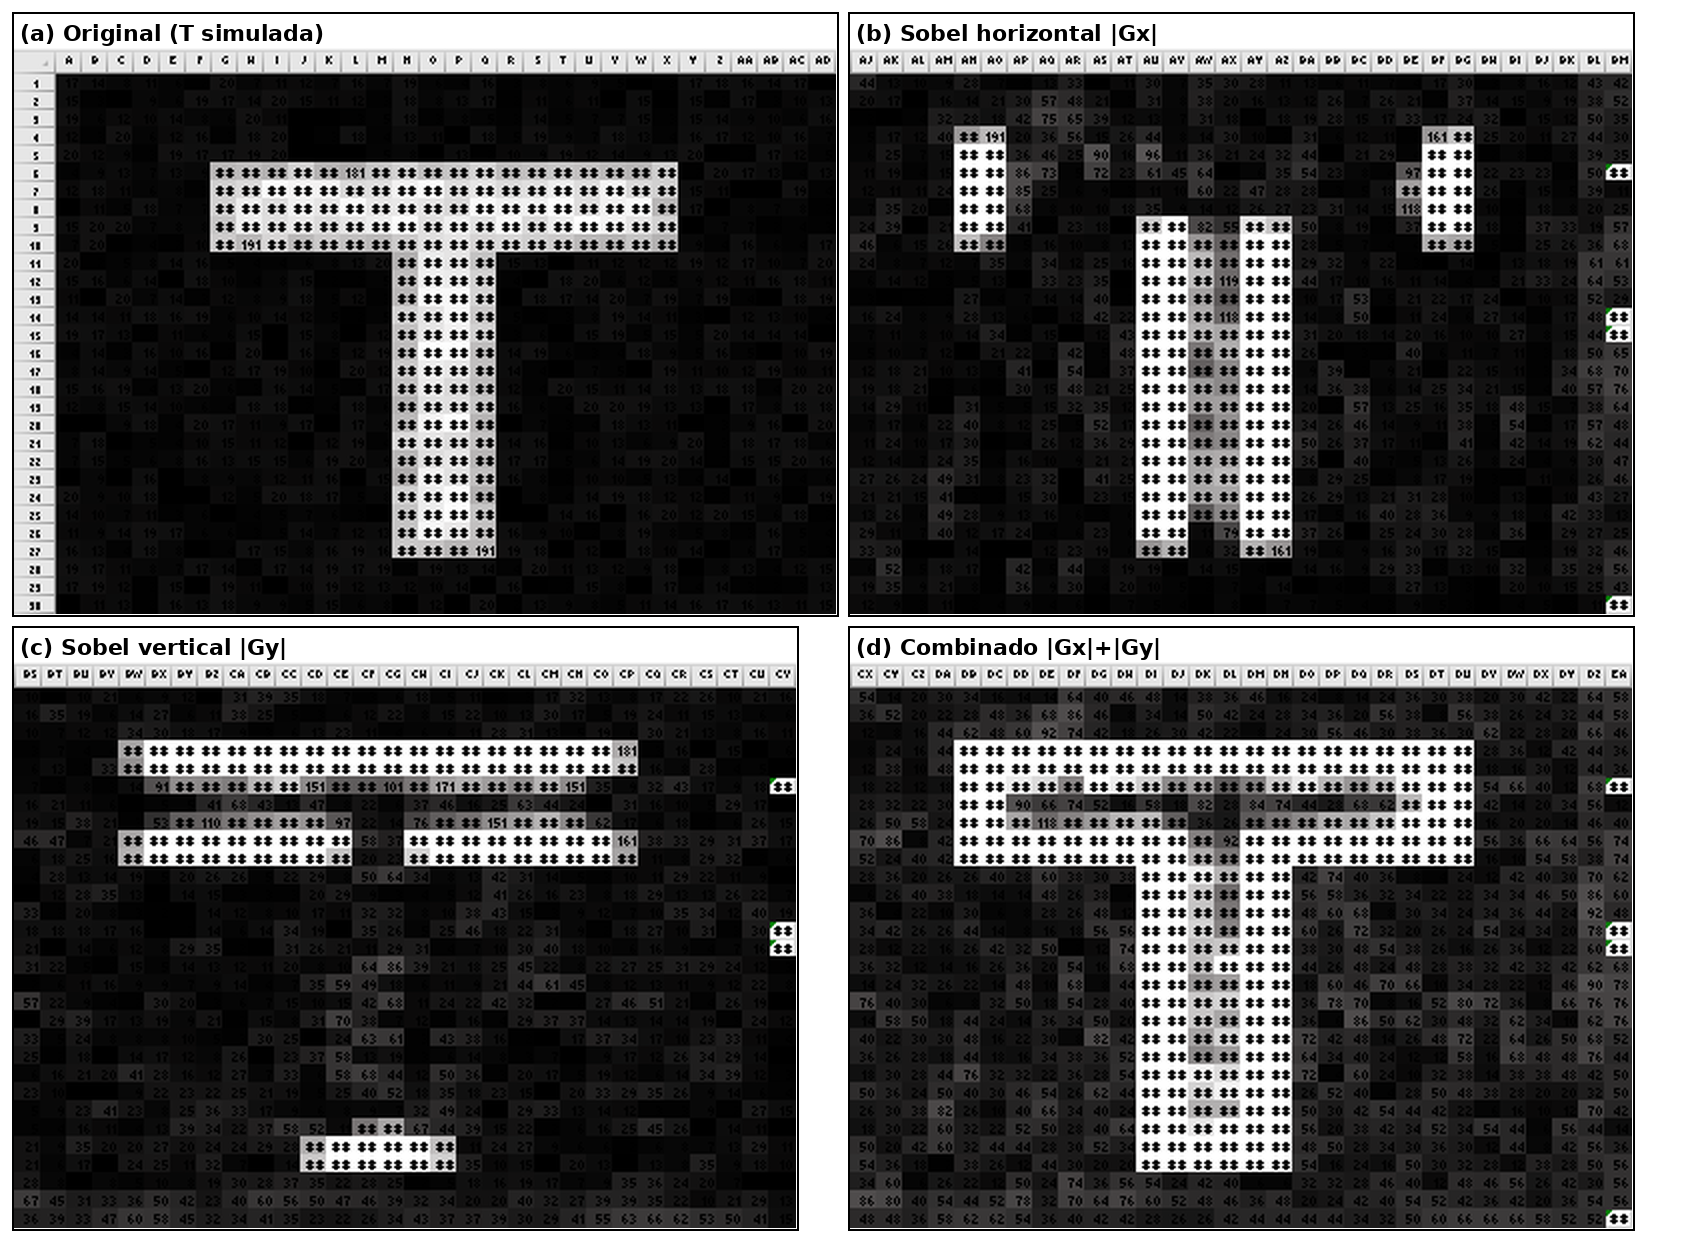
\includegraphics[width=0.95\textwidth]{figuras/reto2_sobel_sin_gaussiano.png}
\caption{Pipeline sin suavizado previo: (a) matriz original generada con
\texttt{ALEATORIO.ENTRE} (fondo 0--10, penumbra de un borde, esquina hasta
255); (b) respuesta de Sobel horizontal; (c) respuesta de Sobel vertical;
(d) magnitud combinada $|G_x|+|G_y|$. Capturas de la hoja de cálculo con
formato condicional en escala de grises.}
\label{fig:reto2-sin-gauss}
\end{figure}

\begin{figure}[ht]
\centering
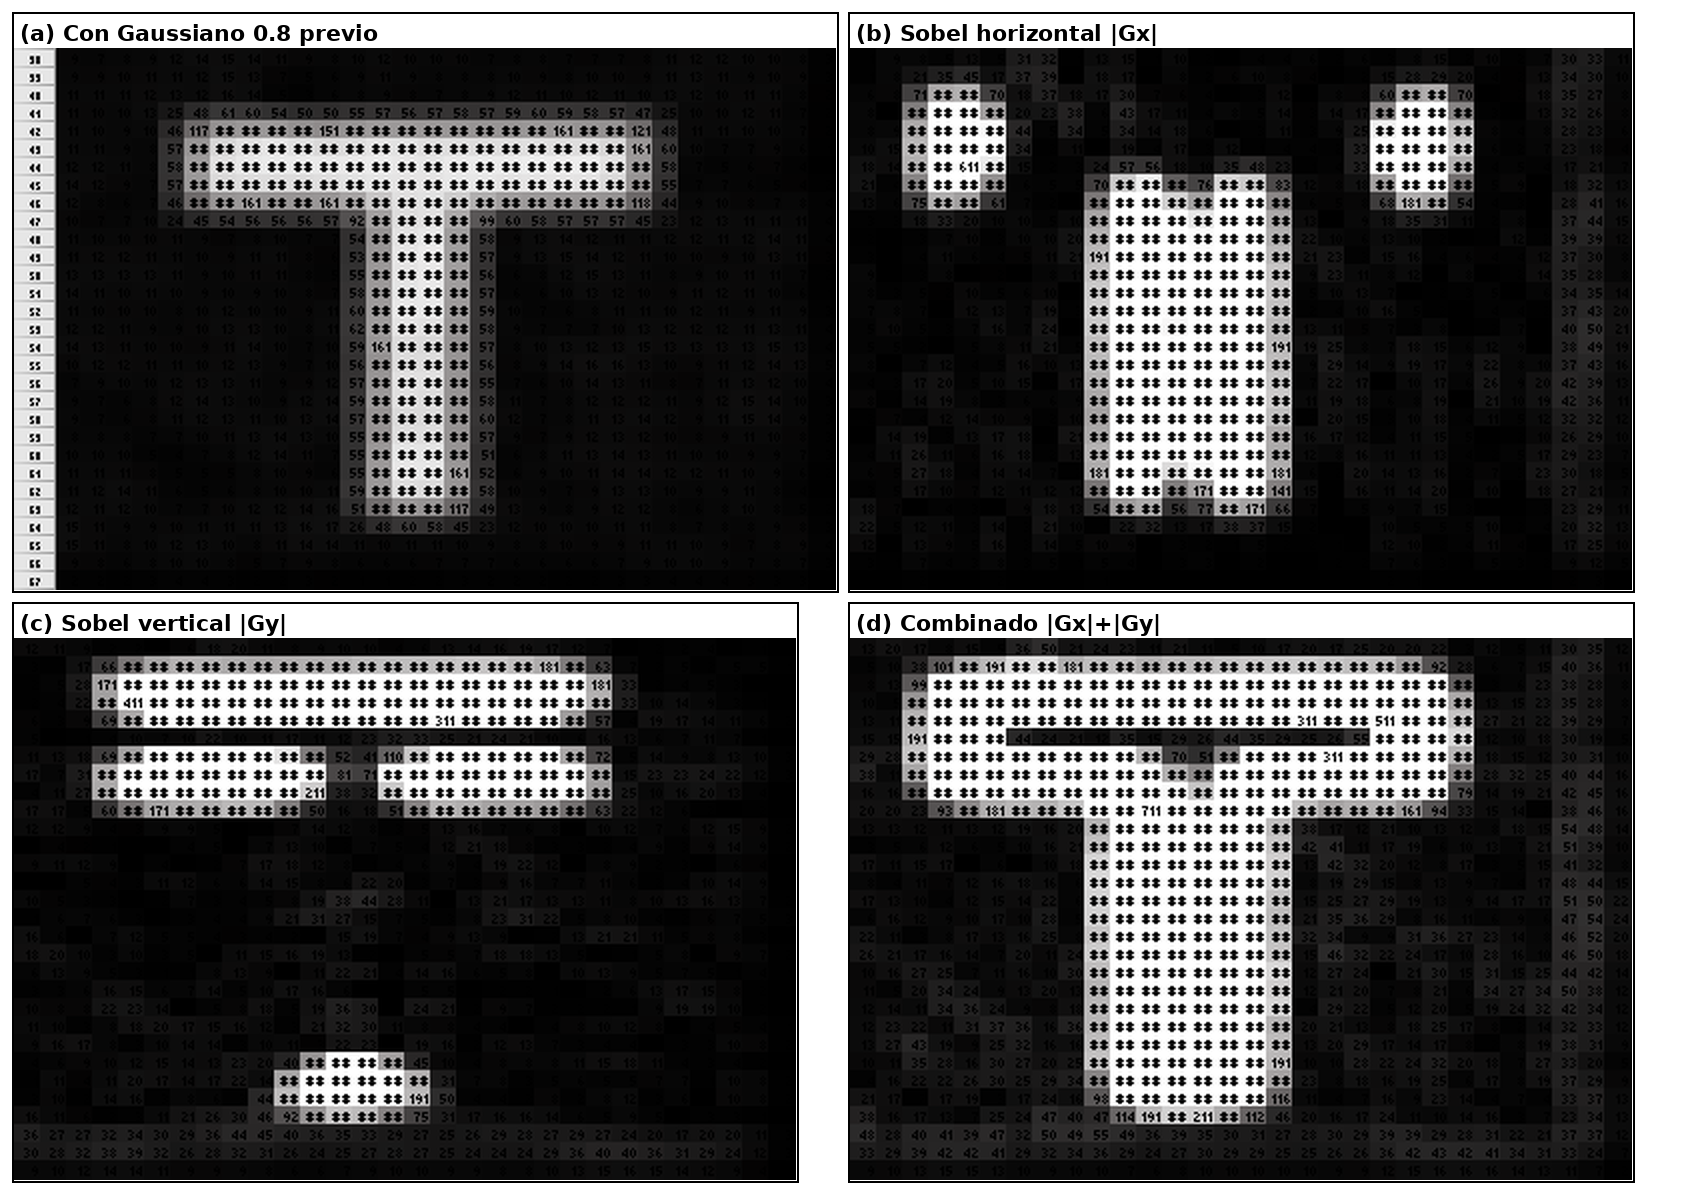
\includegraphics[width=0.95\textwidth]{figuras/reto2_sobel_con_gaussiano.png}
\caption{Mismo pipeline, aplicando primero un suavizado gaussiano
$3\times 3$ ($\sigma\approx 0{,}8$) sobre la matriz original: (a) imagen
suavizada (nótese que conserva el rango 0--255 pero introduce valores
decimales); (b)--(c) respuesta de Sobel horizontal y vertical sobre la
imagen suavizada; (d) magnitud combinada.}
\label{fig:reto2-con-gauss}
\end{figure}

Las Figuras~\ref{fig:reto2-sin-gauss} y \ref{fig:reto2-con-gauss} muestran
el resultado esperado desde la teoría del operador de Sobel: la esquina
simulada produce una respuesta fuerte y de signo opuesto a ambos lados en
el kernel horizontal y en el vertical, y la combinación $|G_x|+|G_y|$
concentra la magnitud de borde alrededor de la esquina, mientras que el
fondo aleatorio de bajo nivel (0--10) queda prácticamente suprimido en
comparación.

\paragraph{¿Por qué la imagen filtrada tiene valores por encima de 255?}
A diferencia de un kernel de suavizado (cuyos pesos suman 1 y por lo tanto
producen un promedio ponderado que nunca puede superar el máximo de la
vecindad), los kernels de Sobel tienen pesos que suman 0 y están diseñados
para responder a \emph{diferencias} de intensidad, no a un promedio. Su
salida es una derivada discreta, no un valor de intensidad acotado: con
pesos máximos de $\pm 4$ por kernel, la respuesta cruda de cada dirección
puede alcanzar en teoría hasta $4\times 255 = 1020$, y la magnitud
combinada $|G_x|+|G_y|$ puede llegar hasta el doble de eso. En la práctica,
en la variante sin suavizado (Figura~\ref{fig:reto2-sin-gauss}d) varias
celdas de la esquina superan la capacidad de columna de la hoja de cálculo
(mostrando \texttt{\#\#\#} en Excel), evidenciando magnitudes de al menos
$\sim$990; en la variante con suavizado gaussiano previo
(Figura~\ref{fig:reto2-con-gauss}d) el máximo observado baja a
$\sim$795. Estos valores no son errores: son la magnitud de un gradiente,
no un pixel, y para desplegarlos como imagen visualizable habría que
normalizarlos o recortarlos (\emph{clipping}) al rango $[0,255]$; aquí se
reportan sin recortar porque el valor crudo es precisamente lo que permite
comparar de forma directa ambos \emph{pipelines}.

Esa comparación deja además un hallazgo cualitativo relevante: suavizar
antes de derivar (Gaussiano $\rightarrow$ Sobel) atenúa la magnitud de la
respuesta de borde (de $\sim$990 a $\sim$795 en este ejemplo), el mismo
compromiso ruido-vs-nitidez de borde que se cuantifica de forma
estadística y formal, con réplicas y prueba de hipótesis, en el Reto 4
(Sección~\ref{sec:reto4}); este reto se limita a establecer el mecanismo y
el método de verificación manual, y deja el análisis estadístico de qué
filtro es preferible para esa sección, donde sí hay razón (ruido impulsivo
con varias réplicas) para aplicar ANOVA.

Durante la verificación de este reto se detectó y corrigió un
error de rango en 14 celdas de las hojas de convolución (`SUMPRODUCT`
aplicado sobre una vecindad de $2\times 3$ en vez de $3\times 3$ en filas
puntuales), documentado junto con su corrección en el historial de control
de versiones del repositorio.

\subsubsection{Análisis y conclusiones}
Los resultados confirman la teoría: la esquina simulada produce una
respuesta fuerte en ambos kernels de Sobel, y suavizar antes de derivar
atenúa esa respuesta (Sección anterior). Aplicar los kernels celda por
celda en una hoja de cálculo, en vez de invocar directamente
\texttt{cv2.Sobel} o \texttt{cv2.filter2D}, obliga a hacer explícita la
operación que esas funciones ejecutan como caja negra: una suma ponderada
sobre una vecindad $3\times 3$ (Algoritmo~\ref{alg:conv3x3}). Esa
comprensión de primer principio es también la que sostiene, en la línea de
investigación doctoral del autor, cualquier decisión de diseño sobre qué
descriptor de bordes/esquinas usar en un \emph{pipeline} de SLAM visual.

\subsection{Reto 3: Colores}
\label{sec:reto3}

\subsubsection{Método}
Se buscó una imagen a color con variedad de colores (la escena sintética
descrita en la Sección~\ref{sec:datos-codigo}) y se leyó con OpenCV. Su
forma (\texttt{shape}), impresa directamente en consola como pide la guía,
es $(1536,\ 2752,\ 3)$ (alto, ancho, 3 canales BGR). Mediante inspección
visual se definieron, por sus coordenadas, 6 regiones de interés (ROI) de
$80\times 80$ píxeles: 5 homogéneas, una por cada color sólido presente en
la escena, y una sexta región deliberadamente heterogénea (mezcla de
colores y texturas), tal como pide la guía. El Algoritmo~\ref{alg:roi}
resume el procedimiento de extracción, dibujo del recuadro sobre la imagen
original, y caracterización estadística por canal.

\begin{algorithm}
\caption{Extracción y caracterización estadística de regiones de interés}
\label{alg:roi}
\begin{algorithmic}[1]
\Require Imagen a color $I$ (canales B, G, R); lista de regiones $R = \{(x_1,y_1,x_2,y_2)\}$
\Ensure Media y desviación estándar por canal para cada región; imagen anotada $I_a$
\State $I_a \gets \text{copia}(I)$
\For{cada región $r=(x_1,y_1,x_2,y_2) \in R$}
    \State $P \gets I[y_1{:}y_2,\, x_1{:}x_2]$ \Comment{parche de la región}
    \For{cada canal $c \in \{B, G, R\}$}
        \State $\mu_{r,c} \gets \text{media}(P[:,:,c])$
        \State $\sigma_{r,c} \gets \text{desv.\ estándar}(P[:,:,c])$
    \EndFor
    \State dibujar\_rectángulo($I_a$, $r$)
\EndFor
\State \Return $\{\mu_{r,c}\}$, $\{\sigma_{r,c}\}$, $I_a$
\end{algorithmic}
\end{algorithm}

\subsubsection{Resultados}
La Tabla~\ref{tab:reto3-roi} resume la media y desviación estándar por
canal BGR de las 6 regiones; la Figura~\ref{fig:reto3-rois} muestra las
regiones dibujadas sobre la imagen original.

\begin{table}[h]
\centering
\caption{Media y desviación estándar por canal (B, G, R) de las 6 regiones de interés.}
\label{tab:reto3-roi}
\begin{tabular}{lccl}
\toprule
Región & Media (B, G, R) & Desv. estándar (B, G, R) & Color dominante \\
\midrule
R1 -- Azul (homog.) & 207.4, 95.5, 1.3 & 1.9, 2.1, 1.2 & Azul saturado \\
R2 -- Verde (homog.) & 103.5, 191.0, 8.9 & 2.7, 2.6, 5.1 & Verde saturado \\
R3 -- Rojo (homog.) & 22.3, 8.0, 204.2 & 3.0, 3.9, 3.1 & Rojo saturado \\
R4 -- Pared (homog.) & 245.1, 241.0, 240.4 & 1.4, 1.4, 1.5 & Blanco/gris claro \\
R5 -- Piso (homog.) & 204.8, 202.1, 194.4 & 3.2, 3.2, 3.3 & Gris claro \\
R6 -- Panel+caja (heterog.) & 150.4, 90.0, 55.3 & \textbf{71.7, 34.5, 61.6} & Mezcla \\
\bottomrule
\end{tabular}
\end{table}

\begin{figure}[h]
\centering
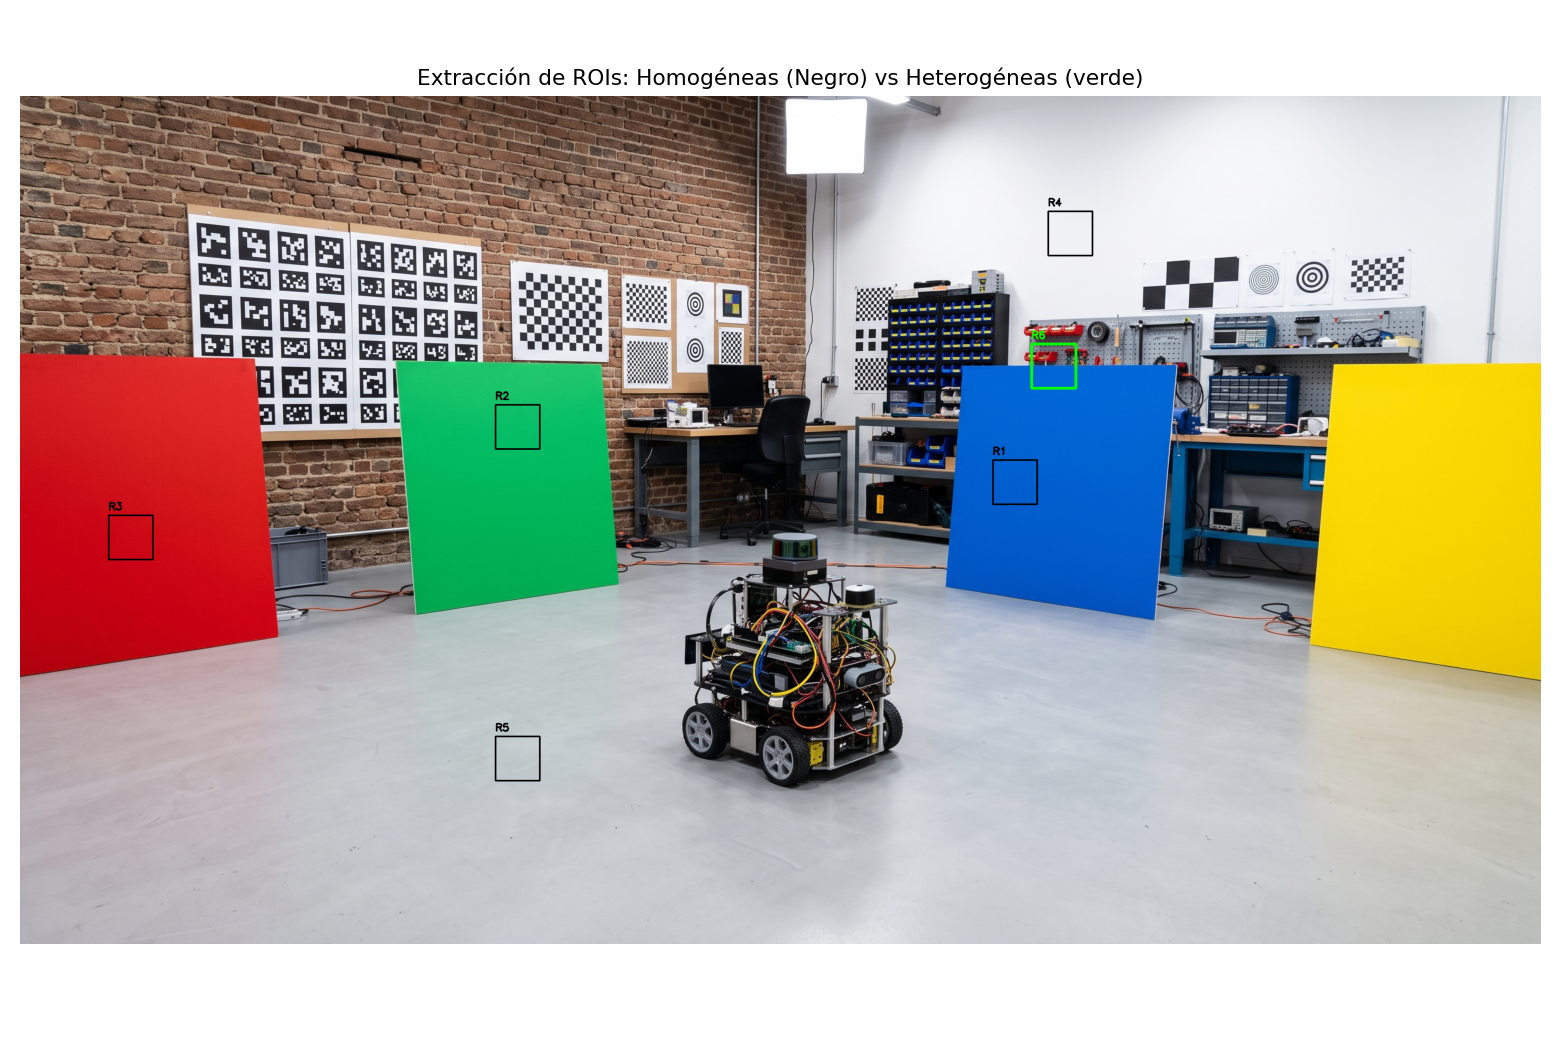
\includegraphics[width=0.9\textwidth]{figuras/reto3_rois_final.png}
\caption{Las 6 regiones de interés dibujadas sobre la imagen original (recuadros negros: regiones homogéneas; recuadro verde: región heterogénea).}
\label{fig:reto3-rois}
\end{figure}

La correspondencia entre medias BGR y el color percibido es la esperada:
R1 (azul) tiene B alto y R muy bajo; R3 (rojo) tiene R alto y B/G bajos; R2
(verde) tiene G dominante; R4 y R5 (pared y piso) tienen los tres canales
altos y muy parecidos entre sí. Las desviaciones estándar de las 5 regiones
homogéneas son todas bajas ($1.2$--$5.1$), mientras que la región 6
(heterogénea) tiene una desviación estándar de 10 a 30 veces mayor
($71.7$ en el canal B, frente a un máximo de $3.2$ en las homogéneas).

\subsubsection{Análisis y conclusiones}
La correspondencia entre las medias BGR y el color percibido, y entre la
desviación estándar y la homogeneidad visual de cada región, confirma que
unos pocos estadísticos por canal bastan para distinguir cuantitativamente
regiones de color sólido de una región mixta, sin necesidad de inspección
visual una vez calculados. Dado el origen sintético de la imagen
(Sección~\ref{sec:datos-codigo}), este reto debe entenderse como una prueba
de concepto del \emph{pipeline} de extracción y caracterización de
regiones (Algoritmo~\ref{alg:roi}); su validación sobre fotografías reales
queda como trabajo futuro (Sección~\ref{sec:conclusiones}). El mismo
principio -- una región con desviación estándar baja es un candidato
estable para seguimiento entre \emph{frames}, mientras que una con
desviación estándar alta es una región ambigua -- es, además, la base de
la caracterización de \emph{landmarks} candidatos en SLAM visual, línea de
trabajo doctoral del autor.

\subsection{Reto 4: Convoluciones para filtrado}
\label{sec:reto4}

\subsubsection{Método}
Sobre una región de $300\times 300$ píxeles recortada de la misma imagen
(Sección~\ref{sec:datos-codigo}), partiendo de la imagen limpia se inyectó
ruido \emph{salt~\&~pepper} al 4\,\% de forma controlada. Siguiendo la
guía, se buscaron e implementaron sin OpenCV cuatro convoluciones
adecuadas para eliminar este tipo de ruido -- media, moda, mediana y
gaussiana, como filtros de suavizado $3\times 3$ (Algoritmo~\ref{alg:conv3x3}
con $f \in \{\text{media}, \text{moda}, \text{mediana}, \text{gaussiana}\}$,
esta última reutilizando el mismo kernel del Reto 2) --, y se compararon
contra las funciones propias de OpenCV (\texttt{cv2.medianBlur},
recomendada por la guía, y \texttt{cv2.GaussianBlur}). Más allá de la
comparación cualitativa pedida por la guía, la calidad de cada filtro se
evaluó también de forma cuantitativa con el índice de similitud
estructural (SSIM) \citep{wang2004ssim} respecto a la imagen sin ruido,
sobre 10 réplicas independientes de ruido por filtro, seguido de un ANOVA
de un factor (el filtro, con 4 niveles) y una prueba post-hoc de Tukey HSD
para identificar qué pares de filtros difieren significativamente entre
sí.

\subsubsection{Resultados}

\begin{table}[h]
\centering
\caption{SSIM medio y varianza por filtro (10 réplicas).}
\label{tab:reto4-anova}
\begin{tabular}{lrr}
\toprule
Filtro & SSIM medio & Varianza \\
\midrule
Media & 0.6272 & 0.000009 \\
Moda & 0.6475 & 0.000031 \\
\textbf{Mediana} & \textbf{0.9255} & 0.000000 \\
Gaussiana & 0.6265 & 0.000009 \\
\bottomrule
\end{tabular}
\end{table}

El ANOVA de un factor resultó altamente significativo: $F = 15801.59$,
$p = 3.40\times 10^{-56}$. La Tabla~\ref{tab:reto4-tukey} presenta las 6
comparaciones post-hoc de Tukey HSD.

\begin{table}[h]
\centering
\caption{Comparaciones post-hoc de Tukey HSD entre los 4 filtros ($\alpha=0.05$).}
\label{tab:reto4-tukey}
\begin{tabular}{lrrl}
\toprule
Comparación & Dif. de medias & $p$-ajustado & ¿Significativa? \\
\midrule
Gaussiana vs.\ Media & 0.0007 & 0.973 & \textbf{No} \\
Gaussiana vs.\ Mediana & 0.2990 & $<0.001$ & Sí \\
Gaussiana vs.\ Moda & 0.0210 & $<0.001$ & Sí \\
Media vs.\ Mediana & 0.2983 & $<0.001$ & Sí \\
Media vs.\ Moda & 0.0203 & $<0.001$ & Sí \\
Mediana vs.\ Moda & $-0.2780$ & $<0.001$ & Sí \\
\bottomrule
\end{tabular}
\end{table}

La Figura~\ref{fig:reto4-filtros} muestra, de forma cualitativa, el mismo
patrón: el ruido desaparece casi por completo con la mediana (manual y
OpenCV), mientras que persiste claramente con media y gaussiana.

\begin{figure}[h]
\centering
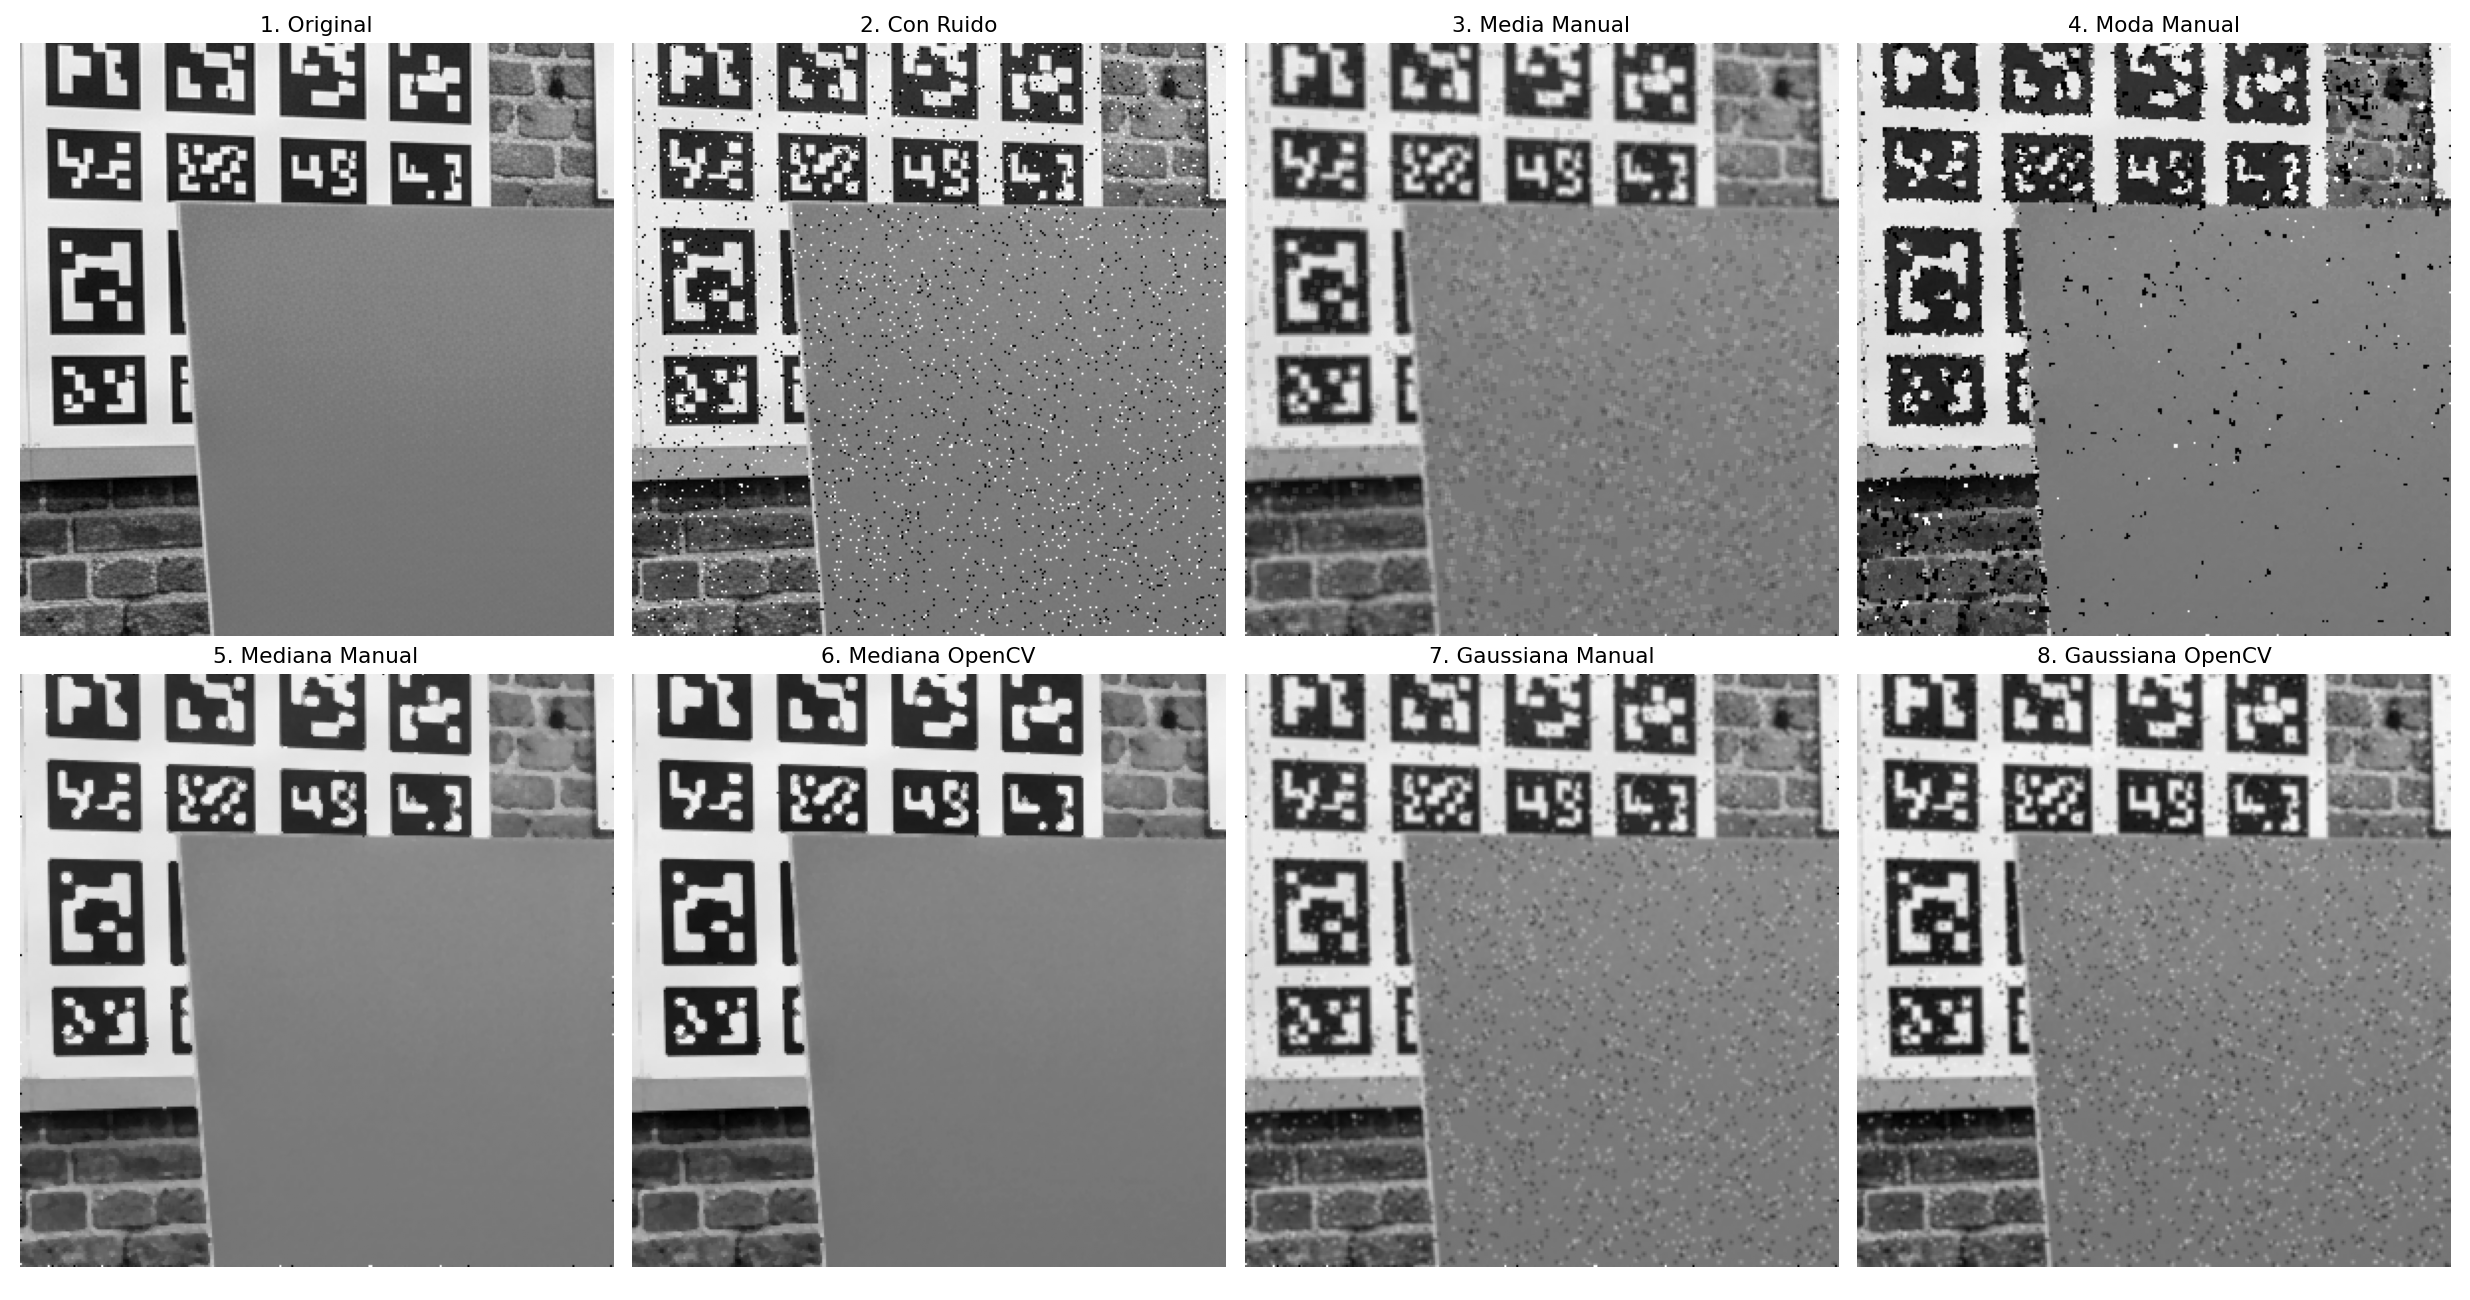
\includegraphics[width=0.95\textwidth]{figuras/reto4_filtros_final.png}
\caption{Comparación visual: original, con ruido, y los 4 filtros manuales frente a sus equivalentes de OpenCV (mediana, gaussiana).}
\label{fig:reto4-filtros}
\end{figure}

Adicionalmente, la Tabla~\ref{tab:reto4-tiempos} compara el costo
computacional de la implementación manual frente a OpenCV.

\begin{table}[h]
\centering
\caption{Tiempo de ejecución: implementación manual vs.\ OpenCV.}
\label{tab:reto4-tiempos}
\begin{tabular}{lrrr}
\toprule
Filtro & Manual (s) & OpenCV (s) & Aceleración \\
\midrule
Mediana & 0.8433 & 0.0001 & $\sim 5770\times$ \\
Gaussiana & 0.1562 & 0.0007 & $\sim 217\times$ \\
\bottomrule
\end{tabular}
\end{table}

\subsubsection{Análisis y conclusiones}
El hallazgo central, pedido por la guía como análisis y conclusión de este
reto, es que \textbf{gaussiana y media son estadísticamente
indistinguibles} ($p=0.973$), y ambas son muy inferiores a la mediana. Esto
es el resultado teóricamente esperado: media y gaussiana son filtros
\emph{lineales} que promedian los valores de la vecindad, incluyendo los
valores extremos ($0$ o $255$) que introduce el ruido \emph{salt~\&~pepper},
de modo que el ruido se esparce en vez de eliminarse; la mediana es un
filtro \emph{no lineal} (estadístico de orden) que, al tomar el valor
central de la vecindad ordenada, descarta directamente esos extremos. Este
resultado, bien conocido en la literatura de procesamiento de imágenes, se
demuestra aquí empíricamente mediante una prueba de hipótesis formal (ANOVA
y Tukey HSD), más allá de lo pedido por la guía, y no solo por inspección
visual. La comparación manual-vs-OpenCV, además, confirma que la
implementación manual reproduce cualitativamente el mismo resultado que
\texttt{cv2.medianBlur} y \texttt{cv2.GaussianBlur}, a un costo
computacional varios órdenes de magnitud mayor.

De los cuatro retos, este es el que más se acerca a un experimento DOE
completo: un factor (el filtro, 4 niveles), una variable de respuesta
cuantitativa (SSIM) medida con réplicas, un ANOVA para establecer si el
factor importa, y una prueba post-hoc para identificar qué niveles difieren
entre sí. Ese mismo esqueleto metodológico (factor = algoritmo SLAM,
niveles = algoritmos candidatos, respuesta = métrica de error/precisión,
réplicas = corridas bajo distintas condiciones) es el que la línea de
investigación doctoral del autor busca formalizar más adelante
(Sección~\ref{sec:conclusiones}).

\section{Discusión}
Tomados en conjunto, los cuatro retos cubren la cadena completa de
operaciones básicas de visión por computador clásica que pedía la
guía: representación matricial de una imagen y caracterización
estadística, manual y vectorizada, de sus valores (Reto 1); el operador de
convolución y los kernels de borde y de suavizado, aplicados celda a celda
para hacerlos explícitos (Reto 2); la representación de color y su
caracterización estadística por región (Reto 3); y el filtrado de ruido
impulsivo, comparando filtros lineales y no lineales tanto de forma
cualitativa como con una prueba de hipótesis formal (Reto 4). En los cuatro
casos la implementación manual (sin librerías especializadas) se verificó
contra su equivalente vectorizado o de OpenCV, lo que permitió confirmar
tanto la corrección de las fórmulas usadas como la magnitud de la ganancia
en desempeño que ofrecen esas librerías.

Del conjunto también se desprende una progresión natural de complejidad
del análisis solicitado: de una comparación de tiempos (Reto 1), a una
verificación de comportamiento esperado por inspección (Reto 2), a una
correspondencia cuantitativa entre estadísticos y percepción visual
(Reto 3), hasta una prueba de hipótesis formal con réplicas para decidir
entre alternativas (Reto 4) -- este último, el más cercano en espíritu al
tipo de comparación de "tratamientos" que estructura un Diseño de
Experimentos.

\section{Conclusiones y trabajo futuro}
\label{sec:conclusiones}
Los cuatro retos de la Guía~1 se resolvieron con implementaciones propias,
verificadas de forma independiente contra sus equivalentes vectorizados o
de OpenCV, y con el análisis y las conclusiones solicitados por la guía en
cada caso. Como trabajo futuro inmediato de esta entrega, se plantea: (1)
diseñar y evaluar, en el Reto 2, un kernel de convolución propio adicional
a los estándar aquí usados (Sobel, gaussiano), tal como sugiere la guía;
(2) validar las conclusiones de los Retos 3 y 4 sobre una fotografía real
además de la escena sintética usada aquí; y (3) explorar formas internas
más complejas (no solo rectangulares) para la matriz del Reto 2.

Más allá de la guía, estos cuatro retos motivan al autor a formalizar, como
parte de su investigación doctoral, un marco metodológico basado en Diseño
de Experimentos (DOE) \citep{montgomery2019design} para evaluar el
desempeño de algoritmos SLAM \citep{cadena2016past,murartal2017orbslam2}.
Varias piezas ya quedaron ensayadas aquí a pequeña escala: medición
reproducible de tiempos y caracterización estadística de variables de
respuesta (Reto 1), comprensión de primer principio de los operadores de
convolución que alimentan cualquier extractor de \emph{features} visual
(Reto 2), caracterización estadística de regiones/\emph{landmarks}
(Reto 3), y sobre todo el esquema de ANOVA y prueba post-hoc de Tukey del
Reto 4, que es en los hechos un prototipo funcional en miniatura del tipo
de experimento -- factor = algoritmo SLAM, niveles = algoritmos candidatos,
respuesta = métrica de error/precisión o tiempo, réplicas = corridas bajo
distintas condiciones -- que se buscará aplicar a algoritmos SLAM
completos en ese trabajo doctoral, quedando la definición formal de esos
factores, niveles y variables de respuesta como una línea de trabajo
separada de esta entrega.

\bibliographystyle{plainnat}
\bibliography{referencias}

\end{document}
